\documentclass{beamer}
\usepackage{graphicx}
\usepackage{listings}
\usepackage{amsfonts}
\usepackage{amsmath}
\usepackage{color}
\usepackage{tikz}
\usepackage{stmaryrd}
\usepackage{mathtools}
\usepackage{bbm}
\usetikzlibrary{shapes.geometric,calc,decorations.text}

\lstdefinelanguage{Kotlin}{
    comment=[l]{//},
    commentstyle={\color{gray}\ttfamily},
    emph={delegate, filter, first, firstOrNull, forEach, lazy, map, mapNotNull, println, return@},
    emphstyle={\color{red}},
    identifierstyle=\color{black},
    keywords={abstract, actual, as, as?, break, by, class, companion, continue, data, do, dynamic, else, enum, expect, false, final, for, fun, get, if, import, in, interface, internal, is, null, object, operator, override, package, private, public, return, sealed, set, super, suspend, this, throw, true, try, typealias, val, var, vararg, when, where, while},
    keywordstyle={\color{blue}\bfseries},
    morecomment=[s]{/*}{*/},
    morestring=[b]",
    morestring=[s]{"""*}{*"""},
    ndkeywords={@Deprecated, @JvmField, @JvmName, @JvmOverloads, @JvmStatic, @JvmSynthetic, Array, Byte, Double, Float, Int, Integer, Iterable, Long, Runnable, Short, String},
    ndkeywordstyle={\color{Orange}\bfseries},
    sensitive=true,
    stringstyle={\color{green}\ttfamily},
    showstringspaces=false,
}

\mode<presentation> { \usetheme{Madrid} }

\title[Array Programming on GF(2^n)]{Probabilistic Array Programming on Galois Fields}
\author[Considine, Guo, Si]{Breandan Considine, Jin Guo, Xujie Si}
\institute[McGill]{
    McGill University, Mila IQIA\\
    \medskip
    \textit{breandan.considine@mail.mcgill.ca}
}
\date{\today}

\begin{document}
    \begin{frame}
        \titlepage
    \end{frame}

    \begin{frame}
        \frametitle{Overview}
        \tableofcontents
    \end{frame}

    \section{Algebraic Parsing}\label{sec:algebraic-parsing}

    %------------------------------------------------------------------------------------------------

    \begin{frame}
        \frametitle{Recap: Context Free Grammars}
        Suppose we have a context free grammar (CFG) $G = \langle V, \Sigma, P, S\rangle$ where $V$ is the set of nonterminals, $\Sigma$ is the terminals, $P: V\times (V \cup \Sigma)^+$ are the productions, $S\in V$ is the start symbol and $+$ is the Kleene plus.\newline\\
        %
        For example, consider the grammar $S \rightarrow S S \mid ( S ) \mid ()$. This represents the language of balanced parentheses, e.g. $(), ()(), (()), ()(()), (()()), (())()\ldots$\newline\\
        %
        Every CFG has a normal form $P^*: V \times (V^2 \mid \Sigma)$, i.e., every production can be refactored into either $v_0 \rightarrow v_1 v_2$ or $v_0 \rightarrow \sigma$, where $v_{0\ldots2}: V$ and $\sigma: \Sigma$, e.g., $[\![S \rightarrow S S \mid ( S ) \mid ()]\!]\Leftrightarrow^*[\![S\rightarrow XR \mid SS \mid LR, L \rightarrow (, R \rightarrow ), X\rightarrow LS]\!]$

        \begin{center}
        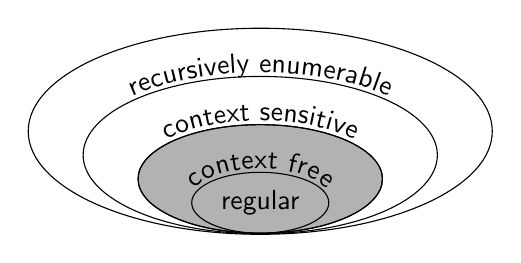
\begin{tikzpicture}[font=\sffamily,breathe dist/.initial=4ex]
            \foreach \X [count=\Y,remember=\Y as \LastY] in
                {regular,context free}
                {\ifnum\Y=1
            \node[ellipse,draw,outer sep=0pt] (F-\Y) {\X};
            \else
            \path[decoration={text along path,
            text={|\sffamily|\X},text align=center,raise=0.3ex},decorate]
        let \p1=($(F-\LastY.north)-(F-\LastY.west)$)
            in (F-\LastY.west) arc(180:0:\x1 and \y1);
            \path let \p1=($([yshift=\pgfkeysvalueof{/tikz/breathe dist}]F-\LastY.north)
            -(F-\LastY.south)$),
            \p2=($(F-1.east)-(F-1.west)$),\p3=($(F-1.north)-(F-1.south)$)
            in ($([yshift=\pgfkeysvalueof{/tikz/breathe dist}]F-\LastY.north)!0.5!(F-\LastY.south)$)
            node[minimum height=\y1,minimum width={\y1*\x2/\y3},
            draw,ellipse,inner sep=0pt, fill=black!30!white] (F-\Y){};
            \fi
            }
            \foreach \X [count=\Y,remember=\Y as \LastY] in
                {regular,context free,context sensitive,recursively enumerable}
                {\ifnum\Y=1
            \node[ellipse,draw,outer sep=0pt] (F-\Y) {\X};
            \else
            \path[decoration={text along path,
            text={|\sffamily|\X},text align=center,raise=0.3ex},decorate]
        let \p1=($(F-\LastY.north)-(F-\LastY.west)$)
            in (F-\LastY.west) arc(180:0:\x1 and \y1);
            \path let \p1=($([yshift=\pgfkeysvalueof{/tikz/breathe dist}]F-\LastY.north)
            -(F-\LastY.south)$),
            \p2=($(F-1.east)-(F-1.west)$),\p3=($(F-1.north)-(F-1.south)$)
            in ($([yshift=\pgfkeysvalueof{/tikz/breathe dist}]F-\LastY.north)!0.5!(F-\LastY.south)$)
            node[minimum height=\y1,minimum width={\y1*\x2/\y3},
            draw,ellipse,inner sep=0pt] (F-\Y){};
            \fi}
        \end{tikzpicture}
        \end{center}
    \end{frame}


    \begin{frame}
        \frametitle{Algebraic Parsing}
        Given a CFG $\mathcal{G} \coloneqq \langle V, \Sigma, P, S\rangle$ in Chomsky Normal Form, we can construct a recognizer $R_\mathcal{G}: \Sigma^n \rightarrow \mathbb{B}$ for strings $\sigma: \Sigma^n$ as follows. Let $\mathcal P(V)$ be our domain, $0$ be $\varnothing$, $\oplus$ be $\cup$, and $\otimes$ be defined as:

        \vspace{-7pt}
        \[
            a \otimes b \coloneqq \{C \mid \langle A, B\rangle \in a \times b, (C\rightarrow AB) \in P\}
        \]

        \noindent We initialize $\mathbf{M}^0_{r,c}(\mathcal{G}, \sigma) \coloneqq \{V \mid c = r + 1, (V \rightarrow \sigma_r) \in P\}$ and search for a matrix $\mathbf{M}^*$ via fixpoint iteration,

        \vspace{-5}
        \[
            \mathbf{M}^* = \begin{pmatrix}
                               \varnothing & \{V\}_{\sigma_1} & \ldots & \ldots & \mathcal{T} \\
                               \varnothing & \varnothing & \{V\}_{\sigma_2} & \ldots & \ldots \\
                               \varnothing & \varnothing & \varnothing & \{V\}_{\sigma_3} & \ldots \\
                               \varnothing & \varnothing & \varnothing & \varnothing & \{V\}_{\sigma_4} \\
                               \varnothing & \varnothing & \varnothing & \varnothing & \varnothing
            \end{pmatrix}
        \]

        \noindent where $\mathbf{M}^*$ is the least solution to $\mathbf{M} = \mathbf{M} + \mathbf{M}^2$. We can then define the recognizer as $R \coloneqq \mathds{1}_{\mathcal{T}}(S) \iff \mathds{1}_{\mathcal{L}(\mathcal{G})}(\sigma)$.
    \end{frame}

    \begin{frame}
        \frametitle{Observations}
        \begin{itemize}
            \item The matrix $\mathbf M^*$ is strictly upper triangular, i.e., nilpotent of degree $n$
            \item The $\otimes$ operator is (sadly) \textit{not} associative
            \item A na\"ive solver has complexity $\mathcal{O}(n^4)$, can be reduced to $\mathcal{O}(n^\omega)$
            \item Recognizer be translated into a parser by storing backpointers
            \item Built-in error recovery: nonempty submatrices = parsable fragments
            \item Can be lowered onto a Boolean tensor $\mathbb{B}^{n\times n \times |V|}$ (Valiant, 1975)
            \item Binarized parser can be efficiently compiled to a SAT solver
            \item Supports sketch-based synthesis in the string or grammar
        \end{itemize}
    \end{frame}

    \begin{frame}
        \frametitle{Binarization}
        \begin{itemize}
            \item We simply encode the characteristic function $\mathds{1}_A: V\rightarrow \mathbb{B}^{|V|}$
            \item $\oplus$ is defined as $\boxplus$ and $\otimes$ is $\boxtimes$, where $\boxplus, \boxtimes: \mathbb{B}^{|V|}\times\mathbb{B}^{|V|} \rightarrow \mathbb{B}^{|V|}$
            \item More sophisticated encodings are known for $\binom{n}{0 \leq k}$ subsets
            \item If density is needed, possible to use the Maculay representation
            \item These operators can be lifted into matrices/tensors in the usual way
            \item Set joins are an active topic of research in SQL query optimization
            \item If you know of a more efficient encoding, I want to talk to you!
        \end{itemize}
    \end{frame}

    \section{IDE Tool}\label{sec:ide}

    \section{Tidyparse tool}\label{sec:tidyparse}

    \section{Usage}\label{sec:usage}

    \begin{frame}
        \frametitle{Usage}
            code goes here
    \end{frame}

    \begin{frame}
        \begin{center}
            \Huge{Learn more at: \\~\\
            \url{http://array22.ndan.co}}
        \end{center}
    \end{frame}

    \begin{frame}
        \frametitle{Special thanks}
        \begin{itemize}
            \begin{center}
                \LARGE{
                    Nghi D. Q. Bui\\
                    Zhixin Xiong\\
                    Jaylene Zhang\\
                    David Yu-Tung Hui\\
                    Fabian Muehlboeck\\
                    Ben Greenman
                }

                \includegraphics[scale=0.3]{../figures/fpt_logo.png}
                \includegraphics[scale=0.2]{../figures/mila_logo.png}
            \end{center}
        \end{itemize}
    \end{frame}
\end{document}